\documentclass{beamer}


% Preamble for english writing
\usepackage[utf8]{inputenc}
\usepackage[T1]{fontenc}
\usepackage{amsmath}
\usepackage{amsfonts}
\usepackage{amssymb}
\usepackage{amsthm}
%\usepackage{algorithmic}
\usepackage{color}
\usepackage{enumerate}
\usepackage{stmaryrd}
\usepackage{hyperref}
\usepackage{graphicx}

%\usepackage{tkz-graph}

%\usepackage[nottoc, notlof, notlot]{tocbibind}

%%%%%%%%%%%%%%%%%%%%%%%%%%%%%%%%%%%%%%%%%%%%%%%%%%%%%%%%%%%%%%%%%%%
%Commandes ajoutées
%%%%%%%%%%%%%%%%%%%%%%%%%%%%%%%%%%%%%%%%%%%%%%%%%%%%%%%%%%%%%%%%%%%

%ensmembles
\newcommand{\N}{\mathbb{N}}
\newcommand{\Z}{\mathbb{Z}}
\newcommand{\Q}{\mathbb{Q}}
\newcommand{\R}{\mathbb{R}}


\newcommand{\intv}[2]{\llbracket #1, #2 \rrbracket} %intervalle d'entiers
\newcommand{\bracket}[1]{{\langle #1 \rangle}} %parenthèses angulaires
\newcommand{\gO}{\mathcal{O}} %grand O
\newenvironment{itemiz}{\renewcommand\labelitemi{$\blacktriangleright$}\begin{itemize}}{\end{itemize}}

\newcommand{\rg}{\text{rg}}
\newcommand{\bad}{\textbf{/!\backslash}}

\newcommand{\crk}{\text{cut-rank}}

\newcommand{\ie}{\emph{i.e.}\ }
\newcommand{\eg}{\emph{e.g.}\ }
\newcommand{\cf}{\emph{c.f.}\ }

% Theorems etc.
\newtheorem{Thm}{Theorem}[section]
\newtheorem{Cor}[Thm]{Corollary}
\newtheorem{Lem}[Thm]{Lemma}
\newtheorem{Pro}[Thm]{Proposition}

\theoremstyle{remark}
\newtheorem{Rem}[Thm]{Remark}
\newtheorem{Not}[Thm]{Notation}
\newtheorem{Exa}[Thm]{Example}

\theoremstyle{definition}
\newtheorem{Def}[Thm]{Definition}

\newcommand{\mytitle}[1]{
\begin{center}
\vspace{7cm}
\hrule
\vspace{0.5cm}
\huge{\textsc{#1}}
\vspace{0.5cm}
\hrule
\vspace{1cm}
\end{center}}



%\usecolortheme{beaver}
\usetheme{Berlin}

\title{\textbf{Evolutionary Computing\\on Turing machines}}
\subtitle{Solving the Busy Beaver Problem}
\author{Jean-Florent Raymond \and Emilio Del Tessandoro}
\institute[Uppsala University]{Uppsala University}
\date{\today}



\begin{document}

\begin{frame}
\titlepage
\end{frame}

\section{Introduction}

\begin{frame}
\frametitle{What is Turing Machine}
%\framesubtitle{}
%they said to say briefly what it is, I think a picture is needed
\begin{figure}
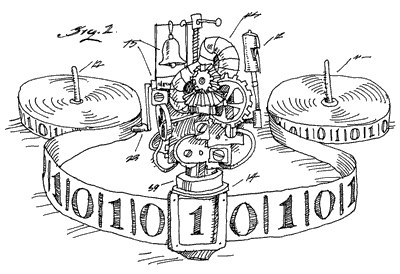
\includegraphics[scale=0.5]{figures/turingMachine.png}
\end{figure}
\end{frame}

\begin{frame}
\frametitle{The Busy Beaver problem}
%\framesubtitle{}
\end{frame}

\begin{frame}
\frametitle{Why it is so hard}
%add another slide with the table, maybe two tables
%one fore the search space size, the other for the number of steps computed by the beavers
\begin{itemize}
\item The size is exponential in $n$, $m$
\item The halting problem, $S$ is not even computable
\item How the ``good'' machines are distributed is not known and not easy
\item $S(n,m)$ grows extremely fast
\end{itemize}
\end{frame}

\section{Possible solutions}

\begin{frame}
\frametitle{Other approaches}
%brute force.. cycles detection.. PSO
\end{frame}

\begin{frame}
\frametitle{Our approach}
%why we used EC
\end{frame}

\begin{frame}
\frametitle{Our solution}
%C++ implementation, TM virtual machine and the EC tool
\end{frame}

\section{Results}

\begin{frame}
\frametitle{What we found}
\end{frame}

\section{Conclusions}

\begin{frame}
\frametitle{Conclusions}
\end{frame}

\end{document}